\chapter{Pragmatics and vagueness}
\label{chapter:vagueness-pragmatics}

This chapter is a brief introduction into the scientific fields associated with the main question. At first I will introduce a linguistic subfield called \textit{pragmatics}, followed by the explanation of the field of (evolutionary) game theory. Then I will go into some discussion about the term "vagueness" in language use and about computer simulations. Some methods of the presented topics are later combined for approaching the main question.

\section{The field of pragmatics}
Human language is an extremely complex communication system, with an 
ever-changing vocabulary and differences between written and spoken language.
Although the use of language is inter-individually different and changing over
time, we are still capable of interpreting certain utterances correctly, even when
the actual semantic meaning might differ from the intended meaning (e.g. in ironic
utterances or exaggerations). In the subfield of linguistics called pragmatics, the way in which contextual cues and language meaning are combined to understand what a speaker meant is studied. In various applications such as e.g. comparison class studies, it can be shown that not only word meaning itself, structural and linguistic knowledge provide meaning, but also the context of an utterance, which is often implicitly referred to \citep[see e.g.][]{tessler2017warm}.\\

In general, the content of so-called "speech-acts" which are uttered by the
speaker or interpreted by the listener in a specific communication situation with
a specific context is analyzed. Context in a communication situation includes physical, mental, social states of the world as well as communicative goals of both, sender and receiver. Pragmatic reasoning, which takes into account this context, can be quantitatively predicted well "by assuming that speakers try to be informative and that listeners use Bayesian inference to recover speakers’ intended referents" \citep{frank2012predicting}, see also \citep{lassiter2013context}.\\

Associated questions could be: What is the question under discussion (QUD) or the topic of the current conversation? In which way are mental representations of the world influencing the communication process? Is it the goal to convey information in a rational way or do factors such as deception or irony play a role?\\

To analyze the content of a specific speech-act, one needs to specify a concrete communication situation which provides answers to the upper questions. Game Theory provides a framework for specifying such situations (here called "games", an explanation will follow in the next section) for further examination.



\section{Evolutionary Game Theory}
\label{sec:egt}

Game theory in general is a branch of applied mathematics for analyzing strategic interactions between individuals (from now on called "agents").
An abstract description of a situation where agents interact with each other in a way that they make certain choices is from now on called a "game". The outcome ("communicative success" or "expected utility") of the interaction for each agent is dependent on the other agent's choices. A simple example for such a game is given below, a version of the so-called "signaling game", discussed first by \cite{lewis2008convention}:\\

Two players, a sender $S$ and a receiver $R$ are trying to maximize their communicative success (i.e. they want to understand each other).
At the beginning, $S$ is given/observing a random world state $w$, this could be the height of a certain object or person. $R$ cannot observe $w$. Then, $S$ chooses a message $m$ to describe the observed state and transmits it to $R$. Based on the observed message, $R$ can now decide for a certain action $a$. In a simple case, the task for $R$ is just to guess the described state $w$. If the guessed state equals the original state, the communication was successful.
A speaker strategy is a function mapping from world states to messages, while a receiver strategy works the other way round, mapping messages to world states (at least in the simple case, where an action $a$ is equal to choosing a certain $w$).\\

While the sets of possible states and messages are usually considered to be
finite in the presented games, we do face the problem that the set of possible
world states and messages are infinite in the natural world and language. A reasonable simplification of the real-world information could look like this:
Depending on the topic, the possible world states are somehow restricted. When
talking about person's heights, we can say for sure that the height "5 meters"
does not apply to any human being, as well as there are no negative heights. 
Even though the space of heights is continuous, the resolution of human perception is limited. This allows for a discrete description of height, while we can assume that is is unrealistic that people can distinguish between heights like 1.810m vs. 1.812m.
Further assumptions on the details of the simulated game will be made in chapter 4.\\

After introducing Game Theory in general, especially when investigating in the evolution of language use, it is also interesting to examine how the outcome of a sender-receiver game correlates with the future use of a certain behavior/strategy in a population of agents. Although the concept of evolution originates from biology, it is still applicable to other domains such as culture and cognition. If some specific conditions are met in the population (e.g. members of the population vary in features, e.g. strategies, which are correlated with "replicative success"), \cite{jager2007evolution} states that "selection, i.e., the spread of successful variants[/strategies] in the population, will be the consequence". In conclusion, 
\begin{quote} 
"[Evolutionary game theory (EGT)] is a mathematical approach to studying how different types of behavior in such games would increase, decrease, die out or prevail in populations of agents who are repeatedly playing the game in question." \citep{franke2014game}
\end{quote}
This is where evolutionary stability and dynamics come in. These two main approaches (see Huttegger and Zollman, 2013) try to explain evolutionary behavior (i.e. the increase/decrease) of certain strategies in populations of individuals. The individuals do use different strategies that lead to different payoffs (from now on referred to as "expected utility (EU)"). More specifically, I will now define the notion of an "evolutionary stable strategy" (ESS) due to \cite{thomas1985evolutionarily}:\\

With: $S$ = set of possible strategies, and $EU(s_1, s_2) = $ EU for a player with strategy $s_1$ playing against a player with strategy $s_2$.\\

Strategy $s_i$ is an ESS, if for all $s_j \neq s_i \in  S$:
\begin{align}
1. EU(s_i, s_i) &\geq EU(s_j, s_i) \quad \textbf{and} \\
2. EU(s_i, s_j) &> EU(s_j, s_j)
\end{align}
The expected utility if both players play strategy $s_i$ must be higher or equal than the EU score of one player playing with strategy $s_i$ and the other one with $s_j \neq s_i$. Also, the EU score of only one player playing strategy $s_j$ (while the other plays with $s_i$) must be higher than the EU score of both players playing strategy $s_j$. If both of these conditions are met, $s_i$ is defined to be an ESS. This definition will be used again in chapter 5, when looking at the simulation results.

\section{Vagueness in language use}
\label{sec:vagueness}

From now on I will often use the notion "\textit{vague} expressions". This chapter aims to clarify the intended meaning of this term. When looking into the literature, a lot of different approaches to the explanation of the term "vagueness" can be found, which makes it difficult to come up with a short but informative definition that suits the needs of this work.\\

One main characteristic of a vague term is the existence of so-called borderline cases, where it's not clear if an object has a certain property $p$ or not. Consider the case $p=$\textit{tall}, like in the example from the beginning. An adult person with a height of 1.20m is definitively not considered as tall, while a 2.20m person would be considered as tall. What about Simon, who is 1.82m? Some might say he is tall, others not, so this would be a borderline case. Beside the pure existence of borderline cases, in many applications, it is also not clear where these borderline cases lie exactly on the relevant scale, which can be considered as some sort of "higher order vagueness".\\

In contrast, a term with a "crisp" meaning would be something like \textit{empty} or \textit{taller than exactly 1.80m}, that unambiguously discriminates two distinct sets of objects, so there are no borderline cases \citep[as in][]{franke2010vagueness}. Most gradable adjectives like \textit{warm} or \textit{good} share this property of being vague. The meaning of these utterances is highly dependent on context and comparison class, as van Rooij pointed out \citep{van2011vagueness}.\\

But what, then, do we make of the contribution from such a word like \textit{tall}? A widespread denotation is a threshold semantics, meaning that the adjective asserts that the relevant property surpasses some point on the respective scale. Example: \textit{tall} means "taller than a certain threshold $\theta_{tall}$". This threshold can be contextually determined, e.g. if the comparison class is common knowledge in the given context. In this case, the sentence "Marc is tall" provides information about the height of Marc, which would be called a descriptive mode of use of the adjective \citep[by][]{barker2002dynamics}. The provided information can be used by a listener for rational inference of a described world state when hearing the word \textit{tall}.
\begin{figure}[!h]
 	\centering
 	\subfloat[Crisp meaning function, according to $P(\theta)$ \newline
    \hspace{\linewidth} in figure (c).\label{subfig:cdf-crisp}]{
 	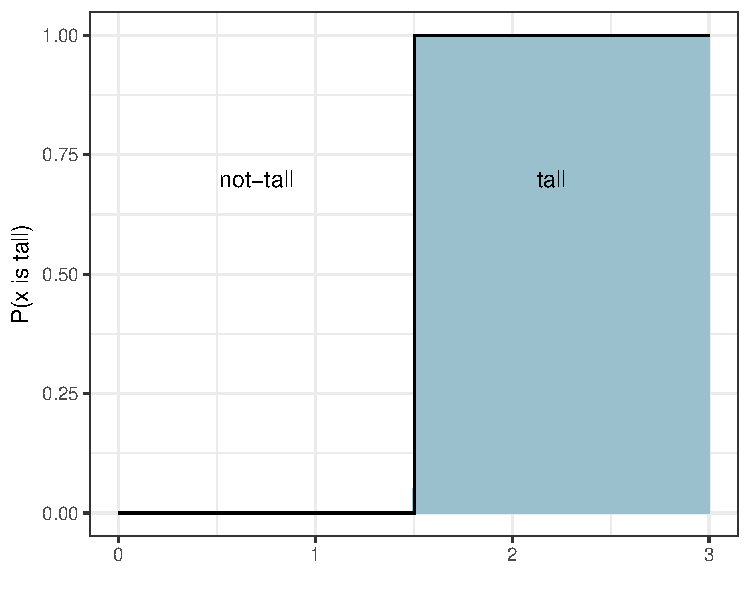
\includegraphics[width=0.5\textwidth]{cdf_crisp.pdf}
 	} 	
 	\subfloat[Vague meaning function with borderline cases, according to $P(\theta)$ in figure (d).\label{subfig:cdf-vague}]{
 	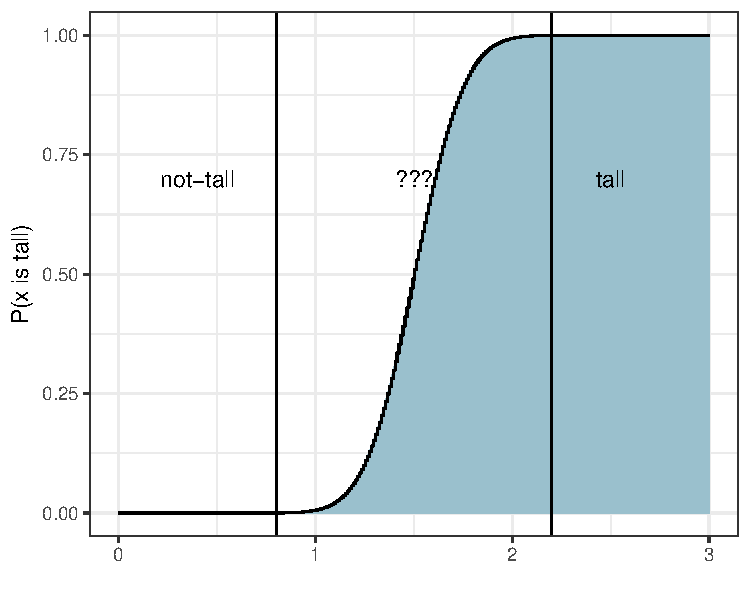
\includegraphics[width=0.5\textwidth]{cdf_vague.pdf}
 	}
 	\\
 	\subfloat[Exact belief about the value of $\theta$.\label{subfig:p-crisp}]{
    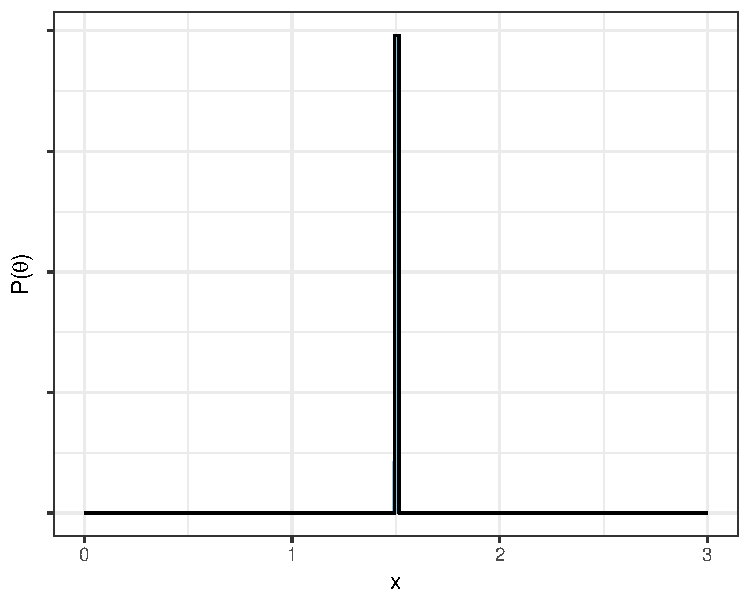
\includegraphics[width=0.5\textwidth]{p_crisp.pdf}
 	}
 	\subfloat[Uncertainty about the exact value of $\theta$.\label{subfig:p-vague}]{
    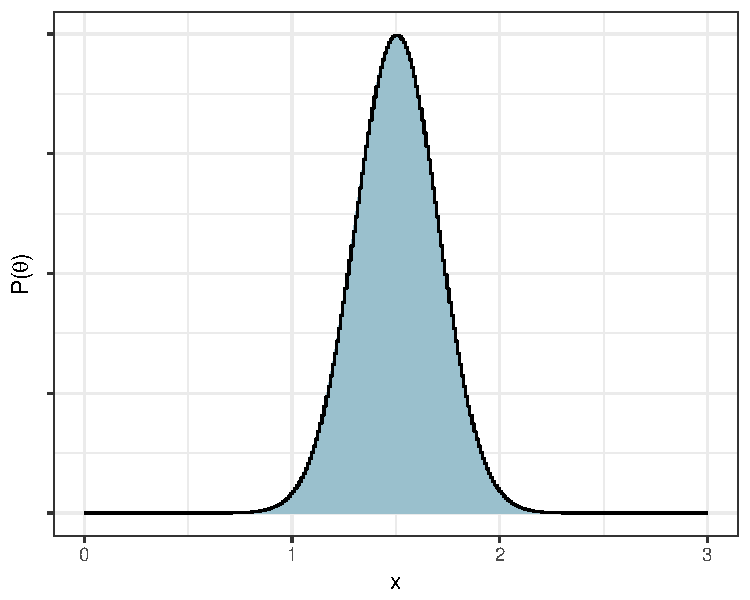
\includegraphics[width=0.5\textwidth]{p_vague.pdf}
 	}
 \caption{Schematic presentation of crisp and vague denotations.\\
 $P$(x is tall) = $\Phi(P(\theta)) \quad (\Phi =$ cumulative density function)}
 \label{figure:meaning}
\end{figure}
Another mode of use is a metalinguistic one: 
When you ask a basketball-player "What counts as \textit{tall} for you as a basketball-player?", and he answers "Phil, who is 2.12m, is tall", this means that his threshold for being tall is below Phil's height in this consideration. 
In this example, the use of the word \textit{tall} "eliminates [...] the possibility that the vague standard of absolute tallness might be greater than the maximal degree of [Phil's] height" \citep{barker2002dynamics}. Therefore, information about the underlying threshold $\theta_{tall}$ is provided, given the height of Marc.\\

As mentioned before, if the threshold is clear, as in "taller than exactly 1,80m", this would be called a crisp denotation instead of a vague one, although it is not referring to one specific world state. With this assumption, "vagueness" can be understood as uncertainty about the exact value of the threshold $\theta$.\\

What this uncertainty means for the semantics of gradable adjectives can be formalized as a probability distribution $P(\theta)$ over the possible values for $\theta$. In Figure \ref{subfig:p-crisp}, all probability mass lies on one point, there is no uncertainty about the value of the threshold. The meaning of the word \textit{tall} then is true (=1) for world states greater than $\theta$ and false (=0) for smaller world states. This "meaning function" is visualized in \ref{subfig:cdf-crisp} and is given by the cumulative density function ($\Phi$) of the the distribution $P(\theta)$. The resulting step function $P(x \textsf{is tall} \mid x) = \Phi(P(\theta))$ can be understood as a model of a crisp denotation. Fig. \ref{subfig:p-vague} shows a Gaussian distribution with mean $\mu$ and standard-deviation $\sigma$ over the possible values for $\theta$, indicating uncertainty about this value. Again, when looking at the cumulative distribution function of $P(\theta)$ in Fig. \ref{subfig:cdf-vague}, the behavior/meaning of a "vague" term is modeled well, in the sense that there are clear cases and borderline cases. It also feels intuitive that the degree to which an object counts as e.g. \textit{tall} increases with its size. This kind of formalization will later be used as an implementation of the semantics in a computer simulation.

\section{Computer simulations for language evolution}
When investigating language evolution or certain properties of language itself, it can be difficult for researchers to perform experiments to  gather data and evidence. It is impossible to change certain aspects of language in an experimental setup, because a person's language representation is deeply grounded within cognition. In many scientific fields, direct observation is not possible and therefore, analytic models and computer simulations might give evidence for developing theories.\\

For setting up a computational model about some property of language, it must be clear which language features are assumed and what features are to be examined. An undesirable direct link between some (global) mechanism in the simulation and the feature to be explained must be avoided. For truly exploring the effects of a certain property, the feature under interest needs to be somehow related to this property, rather than being determined by some (global) mechanism that cannot be observed clearly. Make sure to link an effect to the right cause.\\

Also, there is need for considering configurations that lead to the expected results, as well as configurations that lack the "desired" properties \citep{steels2006experiments}. So called "probabilistic models" are one way of accessing the actual implementation of cognitive processes based on probabilities and statistic inference mechanisms. In a probabilistic generative model there is a formal description about how states of the world are generated or how decisions are made. Often, basic assumptions about the world (e.g. the semantics of a vague term) and causality are stated in this description \citep{probmods2}.An application of probabilistic modeling/cognitive modeling is given in the next chapter, when introducing the Rational Speech Act model.\\

Probabilistic programming languages (PPL) provide a framework for setting up
probabilistic models and perform inference on these.
\textit{webPPL} \citep[by][]{dippl} is my choice of programming language in this work. It is embedded in JavaScript and provides a lot of functions associated with probability-computation, (Bayesian) inference algorithms such as MCMC techniques etc. It also integrates well into R, which I used for data analysis and plotting the results. 